\usepackage{cancel}
\usepackage{xcolor}
\usepackage{amsmath}
\usepackage{amssymb}
\usepackage{hyperref}
\usepackage{caption}
\usepackage[noblocks]{authblk}
\renewcommand*{\Authsep}{, }
\renewcommand*{\Authand}{, }
\renewcommand*{\Authands}{, }
\renewcommand\Affilfont{\tiny}
\usepackage[noblocks]{authblk}
\usepackage{tikz}
\usetikzlibrary{calc}
\usetikzlibrary{arrows}
\usetikzlibrary{arrows.meta}
\usetikzlibrary{shapes}
\usetikzlibrary{positioning}
\usetikzlibrary{shapes.geometric}
\usetikzlibrary{decorations}
\tikzset{>=latex}
\tikzstyle{Arrow} = [->, thick, preaction = {decorate}]
% Define a simple decoration
\tikzstyle{cor} = [-, dotted, preaction = {decorate}]
%\captionsetup{justification=raggedright,singlelinecheck=false}
\captionsetup{justification=raggedright,singlelinecheck=false}
\newcommand{\association}{\tikz[baseline=-0.5ex] \draw[-] (0,0) -- (0.5,0);}
\renewcommand{\rightarrow}{\tikz[baseline=-0.5ex] \draw[-latex] (0,0) to (0.5,0);}
\renewcommand{\leftarrow}{\tikz[baseline=-0.5ex] \draw[-latex-] (0,0) -- (0.5,0);}
\newcommand{\rightarrowblue}{\textcolor{blue}{\rightarrow}}
\newcommand{\rightarrowblueB}{\textcolor{blue}{\to}}
\newcommand{\leftarrowblue}{\textcolor{blue}{\leftarrow}}
\newcommand{\rightarrowred}{\textcolor{red}{\rightarrow}}
\newcommand{\leftarrowred}{\textcolor{red}{\leftarrow}}
\newcommand{\searrowred}{\textcolor{red}{\tikz \draw[-latex] (0,-0) -- (.5,-0.5);}}
\newcommand{\nearrowred}{\textcolor{red}{\tikz \draw[-latex] (0,0) -- (.5,0.5);}}
\newcommand{\rightarrowdotted}{\tikz[baseline=-0.5ex] \draw[dashed, -latex] (0,0) -- (0.5,0);}
\newcommand{\rightarrowdottedblue}{\tikz[baseline=-0.5ex] \draw[blue, dashed, -latex] (0,0) -- (0.5,0);}
\newcommand{\rightarrowdottedred}{\tikz[baseline=-0.5ex] \draw[red, dashed, -latex] (0,0) -- (0.5,0);}
\newcommand{\dottedleftarrowred}{\tikz[baseline=-0.5ex] \draw[red, dashed, latex-] (0,0) -- (0.5,0);}
\newcommand{\dottedleftarrowblue}{\tikz[baseline=-0.5ex] \draw[blue, dashed, latex-] (0,0) -- (0.5,0);}
\newcommand*\circledotted[1]{\tikz[baseline=(char.base)]{\node[shape=circle, inner sep=2pt,draw=black, dashed, thick] (char){$#1$};}}
\newcommand*\circledottedblue[1]{\tikz[baseline=(char.base)]{\node[shape=circle, inner sep=2pt,draw=blue,fill=blue!0, dashed, thick] (char){$#1$};}}
\newcommand*\boxedblue[1]{\tikz[baseline=(char.base)]{
\node[shape=rectangle, , thick, draw=blue, thick, inner sep=2pt,fill=blue!0] (char) {$#1$};}}
\newcommand{\mediation}{A \to \boxed{L} \rightarrowdotted Y}
\newcommand{\xandx}{
\begin{tikzpicture}
\node [rectangle, draw=white] (A) at (0, 0) {X};
\node [rectangle, draw=white] (Y) at (1, 0) {X$^\prime$};
\draw [-latex, draw = white] (A) to (Y);
\end{tikzpicture}
}
\newcommand{\xorx}{
\begin{tikzpicture}
\node [circle, inner sep = 2pt, draw=white] (A) at (0, 0) {X};
\node [circle, inner sep = 2pt, draw=white] (Y) at (1.5, 0) {X$^{\prime}$};
\draw [draw = black] (A) to (Y);
\end{tikzpicture}
}
\newcommand{\xorxorx}{
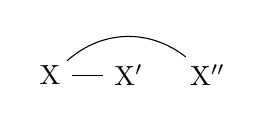
\begin{tikzpicture}
\node [circle, inner sep = 2pt, draw=white] (X) at (0, 0) {X};
\node [circle, inner sep = 2pt, draw=white] (X1) at (1, 0) {X$^{\prime}$};
\node [circle, inner sep = 2pt, draw=white] (X2) at (2, 0) {X$^{\prime \prime}$};
\draw [draw = black] (X) to (X1);
\draw [draw = black, bend left = 40] (X) to (X2);
\end{tikzpicture}
}
\newcommand{\xtox}{
\begin{tikzpicture}
\node [circle, inner sep = 2pt, draw=white] (A) at (0, 0)  {X$_\text{parent}$};
\node [circle, inner sep = 2pt, draw=white] (Y) at (3, 0)  {X$_\text{child}$};
\draw [-latex, draw = black] (A) to (Y);
\end{tikzpicture}
}
\newcommand{\xtoxA}{
\begin{tikzpicture}
\node [circle, inner sep = 2pt, draw=white,  align=center] (A) at (0, 0)  {X$_0$};
\node [circle, inner sep = 2pt, draw=white,  align=center] (Y) at (2, 0)  {X$_1$};
\draw [-latex, draw = black] (A) to (Y);
\end{tikzpicture}
}
\newcommand{\child}{
 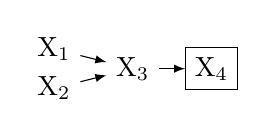
\begin{tikzpicture}
 \node [rectangle, draw=white] (A) at (0, .25) {X$_1$};
 \node [rectangle, draw=white] (L) at (1, 0) {X$_3$};
 \node [rectangle, draw=black] (L1) at (2, 0) {X$_4$};
 \node [rectangle, draw=white] (Y) at (0, -.25) {X$_2$};
 \draw [-latex, draw = black] (A) to (L);
 \draw [-latex, draw = black] (Y) to (L);
 \draw [-latex, draw = black] (L) to (L1);
 \end{tikzpicture}
}
\newcommand{\fork}{
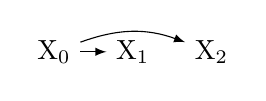
\begin{tikzpicture}
\node [rectangle, draw=white] (L) at (0, 0) {X$_0$};
\node [rectangle, draw=white] (A) at (1, 0) {X$_1$};
\node [rectangle, draw=white] (Y) at (2, 0) {X$_2$};
\draw [-latex, draw = black] (L) to (A);
\draw [-latex, draw = white, dotted] (A) to (Y);
\draw [-latex, bend left=20, draw=black] (L) to (Y);
\end{tikzpicture}
}
\newcommand{\chain}{
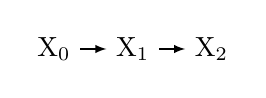
\begin{tikzpicture}
\node [rectangle, draw=white] (A) at (0, 0) {X$_0$};
\node [rectangle, draw=white] (M) at (1, 0) {X$_1$};
\node [rectangle, draw=white] (Y) at (2, 0) {X$_2$};
\draw [-latex, draw = black] (A) to (M);
\draw [-latex, draw = black] (M) to (Y);
\end{tikzpicture}
}
\newcommand{\immorality}{
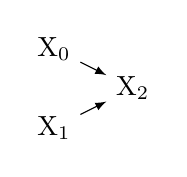
\begin{tikzpicture}
\node [rectangle, draw=white] (A) at (0, .5) {X$_0$};
\node [rectangle, draw=white] (L) at (1, 0) {X$_2$};
\node [rectangle, draw=white] (Y) at (0, -.5) {X$_1$};
\draw [-latex, draw = black] (A) to (L);
\draw [-latex, draw = black] (Y) to (L);
\end{tikzpicture}
}
\newcommand{\network}{
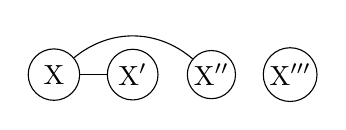
\begin{tikzpicture}
\node [circle, inner sep=3pt, draw=black] (X1) at (0, 0) {X};
\node [circle, inner sep=2pt, draw=black] (X2) at (1, 0) {X$^\prime$};
\node [circle, inner sep=1pt, draw=black] (X3) at (2, 0) {X$^{\prime\prime}$};
\node [circle, inner sep=1pt, draw=black] (X4) at (3, 0) {X$^{\prime\prime\prime}$};
\draw [draw = black] (X1) to (X2);
\draw [bend left=40, draw=black] (X1) to (X3);
\end{tikzpicture}
}
\newcommand{\aandy}{
\begin{tikzpicture}
\node [rectangle, draw=white] (A) at (0, 0) {A$_1$};
\node [rectangle, draw=white] (Y) at (1.5, 0) {Y$_2$};
%\node [draw=none, align=center, font=\tiny] at (1.5,.4) {A and Y are not causally associated};
\draw [-latex, draw = white] (A) to (Y);
\end{tikzpicture}
}
\newcommand{\atoy}{
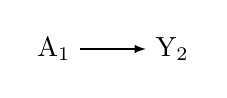
\begin{tikzpicture}
\node [rectangle, draw=white] (A) at (0, 0) {A$_1$};
\node [rectangle, draw=white] (Y) at (1.5, 0) {Y$_2$};
\draw [-latex, draw = black] (A) to (Y);
%\node [draw=none, align=center, font=\tiny] at (1.25,.4) {A and Y are causally associated};
\end{tikzpicture}
}
\newcommand{\descendantA}{
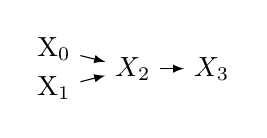
\begin{tikzpicture}
\node [rectangle, draw=white] (A) at (0, .25) {X$_0$};
\node [rectangle, draw=white] (Y) at (0, -.25) {X$_1$};
\node [rectangle, draw=white] (L) at (1, 0) {$X_2$};
\node [rectangle, draw=white] (L1) at (2, 0) {$X_3$};
\draw [-latex, draw = black] (A) -- (L);
\draw [-latex, draw = black] (Y) -- (L);
\draw [-latex, draw = black] (L) -- (L1);
\end{tikzpicture}
}
\newcommand{\atoybiased}{
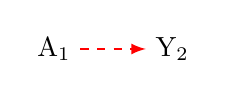
\begin{tikzpicture}
\node [rectangle, draw=white] (A) at (0, 0) {A$_1$};
\node [rectangle, draw=white] (Y) at (1.5, 0) {Y$_2$};
%\node [draw=none, align=center, font=\tiny] at (1.5,.4) {Bias in causal association of A and Y};
\draw [-latex, draw = red, dashed, thick] (A) to (Y);
\end{tikzpicture}
}
\newcommand{\atoybiasedB}{
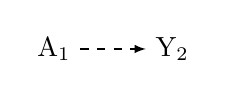
\begin{tikzpicture}
\node [rectangle, draw=white] (A) at (0, 0) {A$_1$};
\node [rectangle, draw=white] (Y) at (1.5, 0) {Y$_2$};
%\node [draw=none, align=center, font=\tiny] at (1.5,.4) {Estimates Direct Effect of A on Y};
\draw [-latex, draw = black, dashed] (A) to (Y);
\end{tikzpicture}
}
\newcommand{\ytoa}{
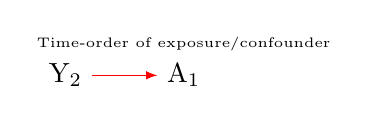
\begin{tikzpicture}
\node [rectangle, draw=white] (A) at (1.5, 0) {A$_1$};
\node [rectangle, draw=white] (Y) at (0, 0) {Y$_2$};
\draw [-latex, red] (Y) to (A);
\node [draw=none, align=center, font=\tiny] at (1.5,.4) {Time-order of exposure/confounder};
\end{tikzpicture}
}
\newcommand{\atwotoyone}{
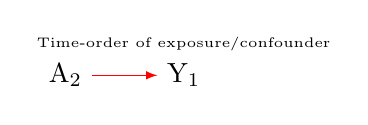
\begin{tikzpicture}
\node [rectangle, draw=white] (A) at (0, 0) {A$_2$};
\node [rectangle, draw=white] (Y) at (1.5, 0) {Y$_1$};
\draw [-latex, draw = red] (A) to (Y);
\node [draw=none, align=center, font=\tiny] at (1.5,.4) {Time-order of exposure/confounder};
\end{tikzpicture}
}
\newcommand{\commoncause}{
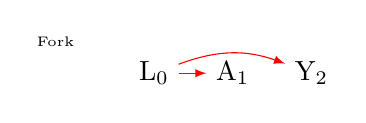
\begin{tikzpicture}
\node [rectangle, draw=white] (L) at (0, 0) {L$_0$};
\node [rectangle, draw=white] (A) at (1, 0) {A$_1$};
\node [rectangle, draw=white] (Y) at (2, 0) {Y$_2$};
\draw [-latex, draw = red] (L) to (A);
\draw [-latex, draw = white, dotted] (A) to (Y);
\draw [-latex, bend left=20, draw=red] (L) to (Y);
\node [draw=none, align=center, font=\tiny] at (-1.25,.4) {Fork};
\end{tikzpicture}
}
\newcommand{\mediator}{
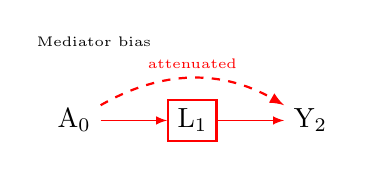
\begin{tikzpicture}
\node [rectangle, draw=white] (A) at (0, 0) {A$_0$};
\node [rectangle, draw=red, thick] (L) at (1.5, 0) {L$_1$};
\node [rectangle, draw=white] (Y) at (3, 0) {Y$_2$};
\draw [-latex, draw = red] (A) to (L);
\draw [-latex, draw = red] (L) to (Y);
\draw [-latex,  bend left=30, draw=red,dashed, thick] (A) to node[pos=0.5, above,draw=none, text = red] {\tiny attenuated} (Y); (Y);
\node [draw=none, align=center, font=\tiny] at (.25,1) {Mediator bias};
\end{tikzpicture}
}
\newcommand{\collider}{
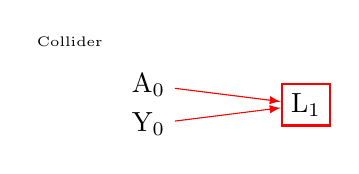
\begin{tikzpicture}
\node [rectangle, draw=white] (A) at (0, .25) {A$_0$};
\node [rectangle,  draw=red, thick] (L) at (2, 0) {L$_1$};
\node [rectangle, draw=white] (Y) at (0, -.25) {Y$_0$};
\draw [-latex, draw = red] (A) to (L);
\draw [-latex, draw = red] (Y) to (L);
\node [draw=none, align=center, font=\tiny] at (-1,.8) {Collider};
\end{tikzpicture}
}
\newcommand{\descendantB}{
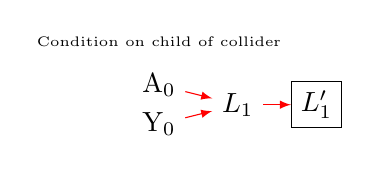
\begin{tikzpicture}
\node [rectangle, draw=white] (A) at (0, .25) {A$_0$};
\node [rectangle, draw=white] (L) at (1, 0) {$L_1$};
\node [rectangle, draw=black] (L1) at (2, 0) {$L'_1$};
\node [rectangle, draw=white] (Y) at (0, -.25) {Y$_0$};
\draw [-latex, draw = red] (A) -- (L);
\draw [-latex, draw = red] (Y) -- (L);
\draw [-latex, draw = red] (L) -- (L1);
\node [draw=none, align=center, font=\tiny] at (0,.8) {Condition on child of collider};
\end{tikzpicture}
}
\newcommand{\mediatorm}{
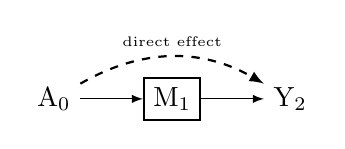
\begin{tikzpicture}
\node [rectangle, draw=white] (A) at (0, 0) {A$_0$};
\node [rectangle, draw=black, thick] (M) at (1.5, 0) {M$_1$};
\node [rectangle, draw = white] (Y) at (3, 0) {Y$_2$};
\draw [-latex, draw = black] (A) to (M);
\draw [-latex, draw = black] (M) to (Y);
\draw [-latex,  bend left=30, draw=black, dashed, thick] (A) to node[pos=0.5, above, draw=none, text = black] {\tiny direct effect} (Y);
\end{tikzpicture}
}
\newcommand{\mbias}{
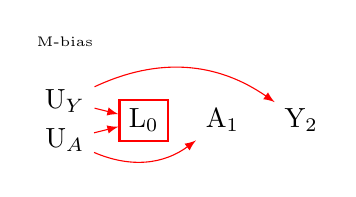
\begin{tikzpicture}
\node [rectangle, draw=white] (UA) at (0, -.25) {U$_A$};
\node [rectangle, draw=white] (UY) at (0, .25) {U$_Y$};
\node [rectangle,  draw=red, thick] (L) at (1, 0) {L$_0$};
\node [rectangle, draw=white] (A) at (2, 0) {A$_1$};
\node [rectangle, draw=white] (Y) at (3, 0) {Y$_2$};
\draw [-latex, draw = red] (UA) to (L);
\draw [-latex, draw = red] (UY) to (L);
\draw [-latex, draw = red, bend right = 30] (UA) to (A);
\draw [-latex, draw = red, bend left = 30] (UY) to (Y);
\node [draw=none, align=center, font=\tiny] at (0,1) {M-bias};
\end{tikzpicture}
}
\newcommand{\mbiasdoomed}{
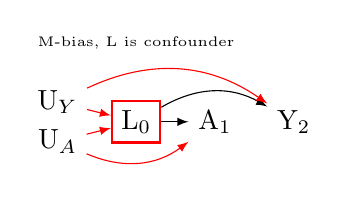
\begin{tikzpicture}
\node [rectangle, draw=white] (UA) at (0, -.25) {U$_A$};
\node [rectangle, draw=white] (UY) at (0, .25) {U$_Y$};
\node [rectangle,  draw=red, thick] (L) at (1, 0) {L$_0$};
\node [rectangle, draw=white] (A) at (2, 0) {A$_1$};
\node [rectangle, draw=white] (Y) at (3, 0) {Y$_2$};
\draw [-latex, draw = black] (L) to (A);
\draw [-latex, draw = black, bend left = 30] (L) to (Y);
\draw [-latex, draw = red] (UA) to (L);
\draw [-latex, draw = red] (UY) to (L);
\draw [-latex, draw = red, bend right = 30] (UA) to (A);
\draw [-latex, draw = red, bend left = 30] (UY) to (Y);
\node [draw=none, align=center, font=\tiny] at (1,1) {M-bias, L is confounder};
\end{tikzpicture}
}
% solutions 
\newcommand{\aandysolution}{
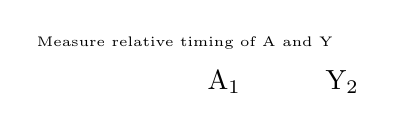
\begin{tikzpicture}
\node [rectangle, draw=white] (A) at (0, 0) {A$_1$};
\node [rectangle, draw=white] (Y) at (1.5, 0) {Y$_2$};
\node [draw=none, align=left, font=\tiny] at (-.5,.5) {Measure relative timing of A and Y};
\draw [-latex, draw = white] (A) to (Y);
\end{tikzpicture}
}
\newcommand{\commoncausesolved}{
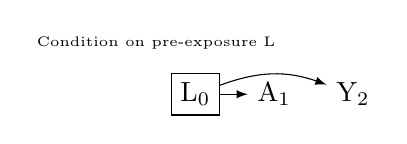
\begin{tikzpicture}
\node [rectangle, draw=black] (L) at (0, 0) {L$_0$};
\node [rectangle, draw=white] (A) at (1, 0) {A$_1$};
\node [rectangle, draw=white] (Y) at (2, 0) {Y$_2$};
\draw [-latex, draw = black] (L) to (A);
\draw [-latex, draw = white, dotted] (A) to (Y);
\draw [-latex, bend left=20, draw=black] (L) to (Y);
\node [draw=none, align=center, font=\tiny] at (-.5,.65) {Condition on pre-exposure L};
\end{tikzpicture}
}
\newcommand{\mbiassolved}{
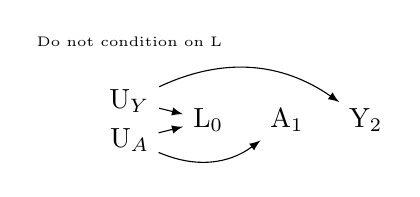
\begin{tikzpicture}
\node [rectangle, draw=white] (UA) at (0, -.25) {U$_A$};
\node [rectangle, draw=white] (UY) at (0, .25) {U$_Y$};
\node [rectangle,  draw=white, thick] (L) at (1, 0) {L$_0$};
\node [rectangle, draw=white] (A) at (2, 0) {A$_1$};
\node [rectangle, draw=white] (Y) at (3, 0) {Y$_2$};
\draw [-latex, draw = black] (UA) to (L);
\draw [-latex, draw = black] (UY) to (L);
\draw [-latex, draw = black, bend right = 30] (UA) to (A);
\draw [-latex, draw = black, bend left = 30] (UY) to (Y);
\node [draw=none, align=center, font=\tiny] at (0,1) {Do not condition on L};
\end{tikzpicture}
}
\newcommand{\commoncausesolvedchild}{
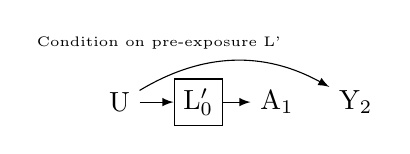
\begin{tikzpicture}
\node [rectangle, draw=white] (U) at (-1, 0) {U};
\node [rectangle, draw=black] (L1) at (0, 0) {L$^{\prime}_0$};
\node [rectangle, draw=white] (A) at (1, 0) {A$_1$};
\node [rectangle, draw=white] (Y) at (2, 0) {Y$_2$};                        
\draw [-latex, draw = black] (U) to (L1);
\draw [-latex, draw = black] (L1) to (A);
\draw [-latex, draw = black, bend left = 30] (U) to (Y);
\node [draw=none, align=center, font=\tiny] at (-.5,.75) {Condition on pre-exposure L'};
\end{tikzpicture}
}
\newcommand{\mbiasdoomedsolved}{
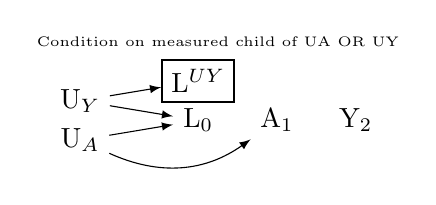
\begin{tikzpicture}
\node [rectangle, draw=white] (UA) at (-1.5, -.25) {U$_A$};
\node [rectangle, draw=white] (UY) at (-1.5, .25) {U$_Y$};
\node [rectangle,  draw=white, thick] (L) at (0, 0) {L$_0$};
\node [rectangle,  draw=black, thick] (L1) at (0, .5) {L$^{UY}$};
\node [rectangle, draw=white] (A) at (1, 0) {A$_1$};
\node [rectangle, draw=white] (Y) at (2, 0) {Y$_2$};
\draw [-latex, draw = black] (UA) to (L);
\draw [-latex, draw = black] (UY) to (L);
\draw [-latex, draw = black, bend right = 30] (UA) to (A);
\draw [-latex, draw = black] (UY) to (L1);
\node [draw=none, font=\tiny] at (.25,1) {Condition on measured child of UA OR UY};
\end{tikzpicture}
}
\newcommand{\effectmodifierA}{
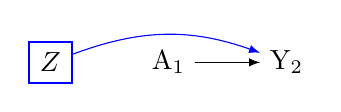
\begin{tikzpicture}
\node [rectangle,  inner sep=4pt,  draw=blue, thick] (Z) at (0,0) {$Z$};
\node [rectangle, draw=white] (A) at (1.5, 0) {A$_1$};
\node [rectangle, draw=white] (Y) at (3, 0) {Y$_2$};
\draw [-latex, draw = blue, bend left = 20] (Z) to (Y);
\draw [-latex, draw = black] (A) to (Y);
\end{tikzpicture}
}
\newcommand{\effectmodifierB}{
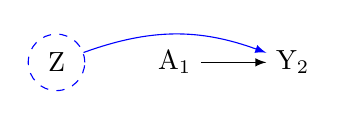
\begin{tikzpicture}
\node [circle,  inner sep=4pt,  draw=blue, dashed] (Z) at (0,0) {Z};
\node [rectangle, draw=white] (A) at (1.5, 0) {A$_1$};
\node [rectangle, draw=white] (Y) at (3, 0) {Y$_2$};
\draw [-latex, draw = blue, bend left = 20] (Z) to (Y);
\draw [-latex, draw = black] (A) to (Y);
\end{tikzpicture}
}
\newcommand{\effectmodifierC}{
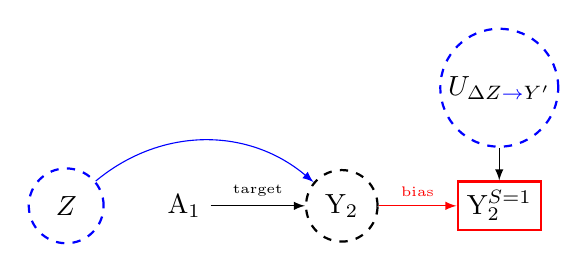
\begin{tikzpicture}
\node [circle, inner sep=6pt, draw=blue,align=left, thick, dashed] (Z) at (0, 0) {$Z$};
\node [rectangle] (A) at (1.5, 0) {A$_1$};
\node [circle, inner sep=4pt,  thick, dashed, draw = black, text=black] (Y) at (3.5,0) {Y$_2$};
\node [circle, inner sep=2pt, draw=blue, text=black, dashed, thick] (US) at (5.5, 1.5) {$U_{\Delta Z \rightarrowblueB Y'}$};
\node [rectangle, draw=black, thick, red, text=black](YS) at (5.5, 0) {Y$_2^{S=1}$};
\draw [-latex, draw=black] (A) to node[pos=0.5, above, draw=none, text = black] {\tiny target}(Y);
\draw [-latex, draw=red] (Y) to node[pos=0.5, above, draw=none, text = red] {\tiny bias}(YS);
\draw [-latex, draw=black] (US) to (YS);
\draw [-latex,bend left=40, blue] (Z) to (Y);
\end{tikzpicture}
}
%measurement
\newcommand{\measurementerroruncorrelated}{
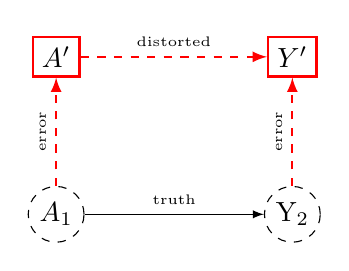
\begin{tikzpicture}
\node [circle, inner sep=2pt, draw=black, dashed] (A) at (0, 0) {$A_1$};
\node [rectangle, draw=red, thick] (A1) at (0, 2) {$A'$};
\node [circle, inner sep=2pt, draw=black, dashed] (Y) at (3, 0) {Y$_2$};
\node [rectangle, draw=red, thick] (Y1) at (3, 2) {$Y'$};
\draw [-latex, draw = red, dashed, thick] (A) to node[pos=0.5, sloped, above, draw=none, text= black] {\tiny error} (A1);
\draw [-latex, draw = red, dashed, thick] (Y) to node[pos=0.5, sloped, above, draw=none, text= black] {\tiny error} (Y1);
\draw [-latex, draw = black] (A) to node[pos=0.5, above, draw=none, text= black] {\tiny truth} (Y);
\draw [-latex, draw = red, dashed, thick] (A1) to node[pos=0.5, sloped, above, draw=none, text=black] {\tiny distorted} (Y1);
\end{tikzpicture}
}
\newcommand{\measurementUNCOR}{
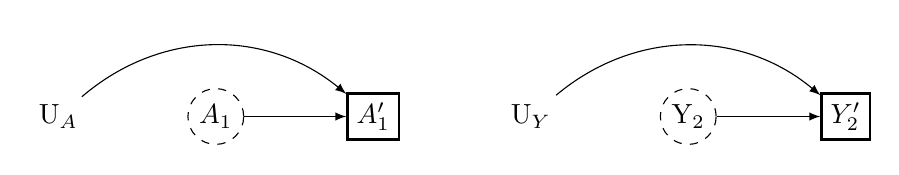
\begin{tikzpicture}
\node [circle, inner sep=2pt, draw=white] (UA) at (0, 0) {U$_{A}$};
\node [circle, inner sep=2pt, draw=black, dashed] (A) at (2, 0) {$A_1$};
\node [rectangle, draw=black, thick] (A1) at (4, 0) {$A'_1$};
\node [rectangle, draw=white] (UY) at (6, 0) {U$_{Y}$};
\node [circle,  inner sep=2pt, draw=black, dashed] (Y) at (8, 0) {Y$_2$};
\node [rectangle, draw=black, thick] (Y1) at (10, 0) {$Y'_2$};
\draw [-latex, draw = black, bend left = 40] (UA) to (A1);
\draw [-latex, draw = black] (A) to (A1);
\draw [-latex, draw = black] (Y) to (Y1);
\draw [-latex, draw = black, bend left = 40] (UY) to (Y1);
\end{tikzpicture}
}
\newcommand{\measurementUCORB}{
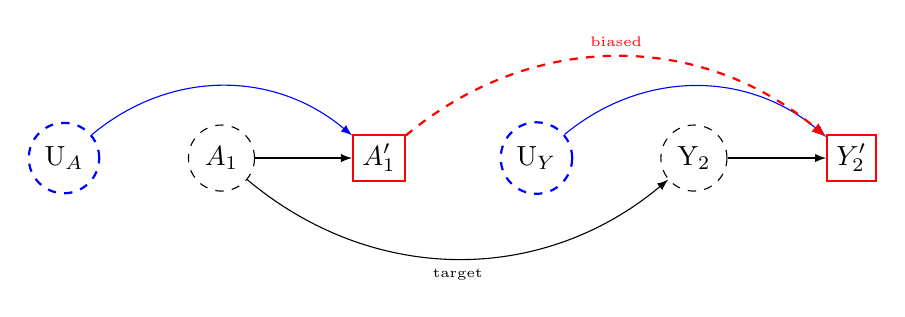
\begin{tikzpicture}
\node [circle, draw=blue, dashed, thick] (UA) at (0, 0) {U$_{A}$};
\node [circle, draw=black, dashed] (A) at (2, 0) {$A_1$};
\node [rectangle, draw=red, thick] (A1) at (4, 0) {$A'_1$};
\node [circle, draw=blue, dashed, thick] (UY) at (6, 0) {U$_{Y}$};
\node [circle, draw=black, dashed] (Y) at (8, 0) {Y$_2$};
\node [rectangle, draw=red, thick] (Y1) at (10, 0) {$Y'_2$};
\draw [-latex, draw = blue, bend left = 40] (UA) to (A1);
\draw [-latex, draw = black] (A) to (A1);
\draw [-latex, draw = black] (Y) to (Y1);
\draw [-latex, draw = blue, bend left = 40] (UY) to (Y1);
\draw [-latex, bend right = 40, draw = black] (A) to node[pos=0.5, below, draw=none] {\tiny target}(Y);
\draw [-latex, bend left = 40, draw = red,  dashed, thick] (A1) to node[pos=0.5, above, draw=none, text= red] {\tiny biased}(Y1);
\end{tikzpicture}
}
\newcommand{\measurementCOR}{
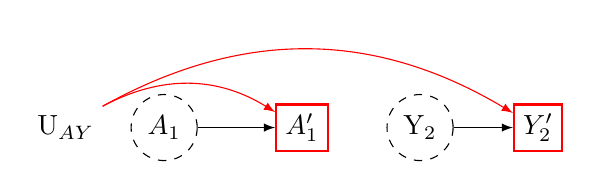
\begin{tikzpicture}
\node [rectangle, draw=white] (U) at (0, 0) {U$_{AY}$};
\node [circle, draw=black, dashed] (A) at (1.25, 0) {$A_1$};
\node [rectangle, draw=red, thick] (A1) at (3, 0) {$A'_1$};
\node [circle, draw=black, dashed] (Y) at (4.5, 0) {Y$_2$};
\node [rectangle, draw=red, thick] (Y1) at (6, 0) {$Y'_2$};
\draw [-latex, draw = red, bend left = 30] (U) to (A1);
\draw [-latex, draw = black] (A) to (A1);
\draw [-latex, draw = red, bend left = 30] (U) to (Y1);
\draw [-latex, draw = black] (Y) to (Y1);
\end{tikzpicture}
}
\newcommand{\measurementDIR}{
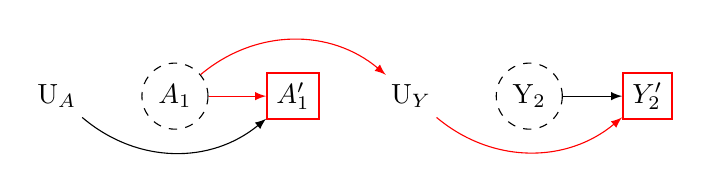
\begin{tikzpicture}
\node [rectangle, draw=white] (UA) at (0, 0) {U$_A$};
\node [circle, draw=black, dashed] (A) at (1.5, 0) {$A_1$};
\node [rectangle,draw=red, thick] (A1) at (3, 0) {$A'_1$};
\node [rectangle, draw=white] (UY) at (4.5, 0) {U$_Y$};
\node [circle, draw=black, dashed] (Y) at (6, 0) {Y$_2$};
\node [rectangle, draw=red, thick] (Y1) at (7.5, 0) {$Y'_2$};
\draw [-latex, draw = black,  bend right = 40] (UA) to (A1);
\draw [-latex, draw = red] (A) to (A1);
\draw [-latex, draw = red, bend left = 40] (A) to (UY);
\draw [-latex, draw =black] (Y) to (Y1);
\draw [-latex, draw = red, bend right = 40] (UY) to (Y1);
\end{tikzpicture}
}
\newcommand{\measurementCORDIR}{
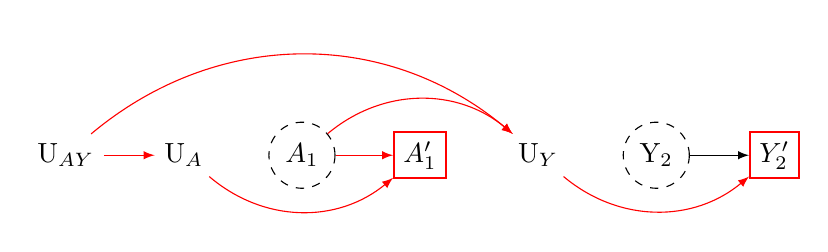
\begin{tikzpicture}
\node [rectangle, draw=white] (UAY) at (0, 0) {U$_{AY}$};
\node [rectangle, draw=white] (UA) at (1.5, 0) {U$_A$};
\node [circle, draw=black, dashed] (A) at (3, 0) {$A_1$};
\node [rectangle, draw=red, thick] (A1) at (4.5, 0) {$A'_1$};
\node [rectangle, draw=white] (UY) at (6, 0) {U$_Y$};
\node [circle, draw=black, dashed] (Y) at (7.5, 0) {Y$_2$};
\node [rectangle, draw=red, thick] (Y1) at (9, 0) {$Y'_2$};
\draw [-latex, draw = red] (UAY) to (UA);
\draw [-latex, draw = red, bend right = 40] (UA) to (A1);
\draw [-latex, draw = red] (A) to (A1);
\draw [-latex, draw = red,bend right = 40] (UY) to (Y1);
\draw [-latex, draw = black] (Y) to (Y1);
\draw [-latex, draw = red, bend left = 40] (A) to (UY);
\draw [-latex, draw = red, bend left = 40] (UAY) to (UY);
\end{tikzpicture}
}
\newcommand{\measurementY}{
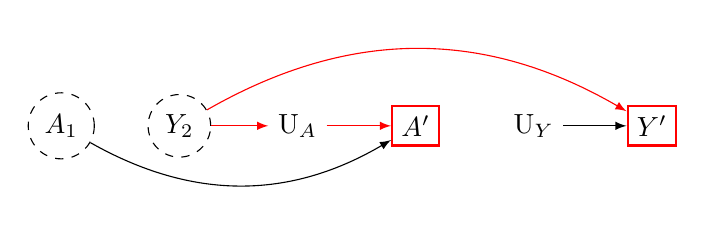
\begin{tikzpicture}
\node [circle, draw=black, dashed] (A) at (0, 0) {$A_1$};
\node [circle, draw=black, dashed] (Y) at (1.5, 0) {$Y_2$};
\node [rectangle, draw=white] (UA) at (3, 0) {U$_A$};
\node [rectangle, draw=red, thick] (A1) at (4.5, 0) {$A'$};
\node [rectangle, draw=white] (UY) at (6, 0) {U$_Y$};
\node [rectangle,  draw=red, thick] (Y1) at (7.5, 0) {$Y'$};
\draw [-latex, draw = red] (Y) to (UA);
\draw [-latex, draw = red] (UA) to (A1);
\draw [-latex, draw = black, bend right = 30] (A) to (A1);
\draw [-latex, draw = black] (UY) to (Y1);
\draw [-latex, draw = red, bend left = 30] (Y) to (Y1);
\end{tikzpicture}
}
\newcommand{\effectmodification}{
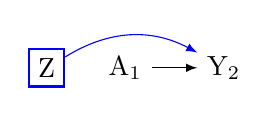
\begin{tikzpicture}
\node [rectangle,thick, draw=blue] (Z) at (-1,0) {Z};
\node [rectangle, draw=white] (A) at (0, 0) {A$_{1}$};
\node [rectangle, draw=white] (Y) at (1.25, 0) {Y$_{2}$};
\draw [-latex, draw=black] (A) to (Y);
\draw [-latex, bend left, draw=blue] (Z) to (Y);
\end{tikzpicture}
}
\newcommand{\effectmodificationunconditioned}{
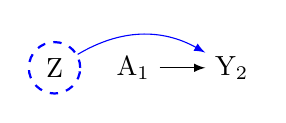
\begin{tikzpicture}
\node [rectangle, draw=white] (A) at (0, 0) {A$_{1}$};
\node [rectangle, draw=white] (Y) at (1.25, 0) {Y$_{2}$};
\node [circle, dashed, thick, draw=blue] (Z) at (-1,0) {Z};
\draw [-latex, draw=black] (A) to (Y);
\draw [-latex, bend left, draw=blue] (Z) to (Y);
\end{tikzpicture}
}
\newcommand{\directeffectmodification}{
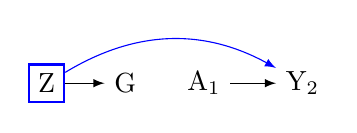
\begin{tikzpicture}
\node [rectangle, draw=white] (A) at (0, 0) {A$_{1}$};
\node [rectangle, draw=white] (Y) at (1.25, 0) {Y$_{2}$};
\node [rectangle, draw=blue, thick] (Z) at (-2,0) {Z};
\node [rectangle, draw=white] (G) at (-1, 0) {G};
\draw [-latex, draw=black] (A) to (Y);
\draw [-latex, bend left, draw=blue] (Z) to (Y);
\draw [-latex, draw = black] (Z) to (G);
\end{tikzpicture}
}
\newcommand{\indirecteffectmodification}{
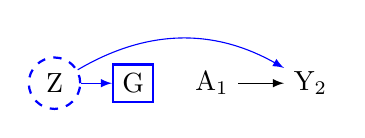
\begin{tikzpicture}
\node [rectangle, draw=white] (A) at (0, 0) {A$_{1}$};
\node [rectangle, draw=white] (Y) at (1.25, 0) {Y$_{2}$};
\node [circle,dashed,draw=blue, thick] (Z) at (-2,0) {Z};
\node [rectangle, draw=blue, thick] (G) at (-1, 0) {G};
\draw [-latex, draw=black] (A) to (Y);
\draw [-latex, bend left, draw=blue] (Z) to (Y);
\draw [-latex, draw = blue] (Z) to (G);
\end{tikzpicture}
}
\newcommand{\indirecteffectmodificationB}{
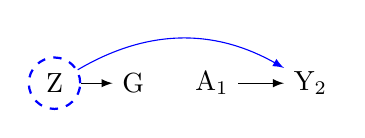
\begin{tikzpicture}
\node [rectangle, draw=white] (A) at (0, 0) {A$_{1}$};
\node [rectangle, draw=white] (Y) at (1.25, 0) {Y$_{2}$};
\node [circle, draw=blue, dashed, thick] (Z) at (-2,0) {Z};
\node [rectangle, draw=white, dashed] (G) at (-1, 0) {G};
\draw [-latex, draw=black] (A) to (Y);
\draw [-latex, bend left, draw=blue] (Z) to (Y);
\draw [-latex, draw = black] (Z) to (G);
\end{tikzpicture}
}
\newcommand{\collidereffectmodification}{
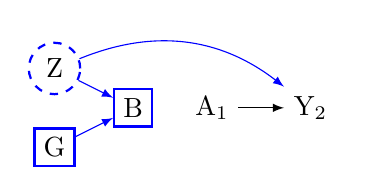
\begin{tikzpicture}
\node [rectangle, draw=white] (A) at (0, 0) {A$_{1}$};
\node [rectangle, draw=white] (Y) at (1.25, 0) {Y$_{2}$};
\node [circle, dashed, thick, draw=blue] (Z) at (-2, .5) {Z};
\node [rectangle, thick, draw=blue, thick] (G) at (-2, -.5) {G};
\node [rectangle, thick, draw=blue] (B) at (-1,0) {B};
\draw [-latex, draw=black] (A) to (Y);
\draw [-latex, bend left, draw=blue] (Z) to (Y);
\draw [-latex, draw=blue] (Z) to (B);
\draw [-latex, draw=blue] (G) to (B);
\end{tikzpicture}
}
\newcommand{\childeffectmodification}{
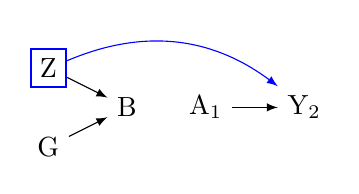
\begin{tikzpicture}
\node [rectangle, draw=white] (A) at (0, 0) {A$_{1}$};
\node [rectangle, draw=white] (Y) at (1.25, 0) {Y$_{2}$};
\node [rectangle, thick, draw=blue] (Z) at (-2, .5) {Z};
\node [rectangle, draw=white] (G) at (-2, -.5) {G};
\node [rectangle, draw=white] (B) at (-1,0) {B};
\draw [-latex, draw=black] (A) to (Y);
\draw [-latex, bend left, draw=blue] (Z) to (Y);
\draw [-latex, draw=black] (Z) to (B);
\draw [-latex, draw=black] (G) to (B);
\end{tikzpicture}
}
\renewcommand*{\restriction}{
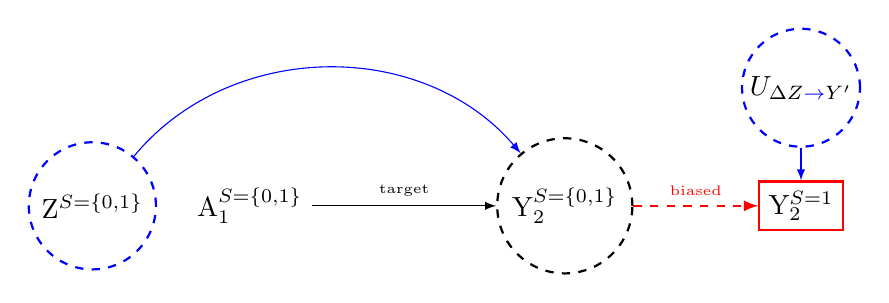
\begin{tikzpicture}
\node [circle, thick, draw=blue, dashed, thick] (Z) at (0, 0) {Z$^{S=\{0,1\}}$};
\node [rectangle, draw=white] (A) at (2, 0) {A$_1^{S=\{0,1\}}$};
\node [circle, draw=black, dashed, thick] (Y) at (6,0) {Y$_2^{S=\{0,1\}}$};
\node [rectangle, draw=red, thick](YS) at (9, 0) {Y$_2^{S=1}$};
\node [circle, inner sep = 2pt, draw=blue,dashed,thick] (US) at (9,1.5) {$U_{\Delta Z \rightarrowblueB Y'}$};
\draw [-latex, draw = red, dashed, thick] (Y) to  node[pos=0.5, draw=none, above, text= red] {\tiny biased }(YS);
\draw [-latex, bend left=50, draw=blue] (Z) to node[pos=0.5, draw=none, above, text= black] {\tiny } (Y);
\draw [-latex, draw=black] (A) to node[pos=0.5, draw=none, above, text= black] {\tiny target}(Y);
\draw [-latex, draw = blue] (US) to (YS);
\end{tikzpicture}
}
\newcommand{\restrictionE}{
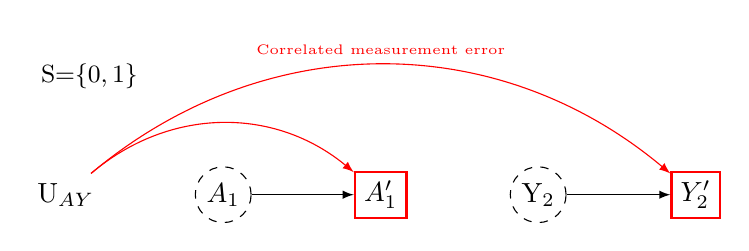
\begin{tikzpicture}
\node [draw=none, font = \small]  (S) at (.3, 1.5) {S=$\{0,1\}$};
\node [rectangle, draw=white] (U) at (0, 0) {U$_{AY}$};
\node [circle, inner sep=2pt, draw=black, dashed] (A) at (2, 0) {$A_1$};
\node [rectangle, draw=red, thick] (A1) at (4, 0) {$A'_1$};
\node [circle, inner sep=2pt, draw=black, dashed] (Y) at (6, 0) {Y$_2$};
\node [rectangle, draw=red, thick] (Y1) at (8, 0) {$Y'_2$};
\draw [-latex, draw = red, bend left = 40] (U) to (A1);
\draw [-latex, draw =black] (A) to (A1);
\draw [-latex, draw = red, bend left = 40] (U) to node[pos=0.5, sloped, above, draw=none, text = red]{\tiny Correlated measurement error}(Y1);
\draw [-latex, draw = black] (Y) to (Y1);
\end{tikzpicture}
}
\newcommand{\restrictionF}{
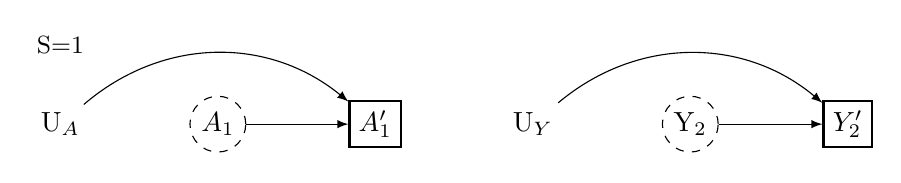
\begin{tikzpicture}
\node [draw=none, font = \small]  (S) at (0, 1) {S=1};
\node [circle, inner sep=2pt, draw=white] (UA) at (0, 0) {U$_{A}$};
\node [circle, inner sep=2pt, draw=black, dashed] (A) at (2, 0) {$A_1$};
\node [rectangle, draw=black, thick] (A1) at (4, 0) {$A'_1$};
\node [rectangle, draw=white] (UY) at (6, 0) {U$_{Y}$};
\node [circle, inner sep=2pt, draw=black, dashed] (Y) at (8, 0) {Y$_2$};
\node [rectangle, draw=black, thick] (Y1) at (10, 0) {$Y'_2$};
\draw [-latex, draw = black, bend left = 40] (UA) to (A1);
\draw [-latex, draw = black] (A) to (A1);
\draw [-latex, draw = black] (Y) to (Y1);
\draw [-latex, draw = black, bend left = 40] (UY) to (Y1);
\end{tikzpicture}
}
\newcommand{\restrictionG}{
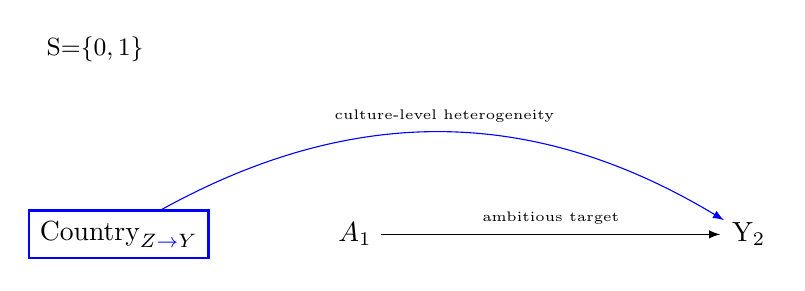
\begin{tikzpicture}
\node [draw=none, font = \small]  (S) at (-.3, 2.35) {S=$\{0,1\}$};
\node [rectangle, inner sep=4pt, draw=blue, thick] (Z) at (0, 0)  {${ \text{Country}_{Z \rightarrowblueB Y}}$};
\node [rectangle, draw = white] (A) at (3, 0) {$A_1$};
\node [circle, inner sep=2pt, draw=white] (Y) at (8, 0) {Y$_2$};
\draw [-latex, draw = blue, bend left = 30] (Z) to node[pos=0.5, above, draw=none, text = black]{\tiny culture-level heterogeneity} (Y);
\draw [-latex, draw = black] (A) to node[pos=0.5, above, draw=none, text = black]{\tiny ambitious target}(Y);
\end{tikzpicture}
}
\newcommand{\restrictionGG}{
\begin{tikzpicture}
\node [draw=none, font = \small] (S) at (-.5, 2.35) {S=$\{0,1\}$};
\node [circle, inner sep=2pt, draw=blue, thick, dashed] (Z) at (0, 0)  {$ \text{Country}_{Z \rightarrowblueB Y}$};
\node [rectangle, draw = white] (A) at (3, 0) {$A_1$};
\node [circle, inner sep=2pt, draw=white] (Y) at (8, 0) {Y$_2$};
\draw [-latex, draw = blue, bend left = 20] (Z) to node[pos=0.5, above, draw=none, text = black]{\tiny culture-level heterogeneity} (Y);
\draw [-latex, draw = black] (A) to node[pos=0.5, above, draw=none, text = black]{\tiny ambitious target}(Y);
\end{tikzpicture}
}
\newcommand{\restrictionGGG}{
\begin{tikzpicture}
\node [draw=none, font = \small] (S) at (0, 1.35) {S=$\{0,1\}$};
\node [circle, inner sep=2pt, draw=blue, dashed, thick] (U) at (0, 0) {$U_{ZY}$};
\node [rectangle, inner sep=2pt, draw=blue, thick] (Z) at (4, 0)  {$ \text{Country}_{Z \rightarrowblueB Y}$};
\node [rectangle, draw = white] (A) at (6, 0) {$A_1$};
\node [circle, inner sep=2pt, draw=black, dashed] (Y) at (10, 0) {Y$_2$};
\node [rectangle, draw=red, thick] (Y1) at (14, 0) {$Y'_2$};
\draw [-latex, draw = blue] (U) to  node[pos=0.5,above, draw=none, text = black]{\tiny } (Z);
\draw [-latex, draw = blue, bend left = 30, dashed, thick] (U) to  node[pos=0.5,above, draw=none, text = black]{\tiny biased effect-modifier heterogeneity} (Y1);
\draw [-latex, draw = red,  dashed, thick] (Y) to node[pos=0.5, above, draw=none, text = red]{\tiny biased ATE}(Y1);
\draw [-latex, draw = blue, bend right = 20] (Z) to node[pos=0.5, below, draw=none, text = black]{\tiny target ATE} (Y);
\draw [-latex, draw = black] (A) to node[pos=0.5, above, draw=none, text = black]{\tiny target}(Y);
\end{tikzpicture}
}
\newcommand{\restrictionH}{
\begin{tikzpicture}
\node [draw=none, font = \small] (S) at (0, 1) {S=1};
\node [circle, inner sep=4pt, draw=blue, dashed] (Z) at (0, 0) {$Z$};
\node [rectangle, draw=white] (A) at (2, 0) {$A_1$};
\node [rectangle, draw=white] (Y) at (6, 0) {Y$_2$};
\draw [-latex, draw = blue, bend left = 30] (Z) to (Y);
\draw [-latex, draw = black] (A) to node[pos=0.5, above, draw=none, text = black]{\tiny modest target}(Y);
\end{tikzpicture}
}
\newcommand{\attritionB}{
\begin{tikzpicture}
\node [rectangle, draw=white] (U1) at (0,1) {U1};
\node [rectangle, draw=white] (U2) at (0,-1) {U2};
\node [rectangle, draw=black, align=left] (S) at (1, 0) {$S = 1$};
\node [rectangle, draw=white] (A) at (2, 0) {A$_{1}$};
\node [rectangle, draw=white] (Y) at (3, 0) {Y$_{2}$};
\draw [-latex, draw=red] (U1) to (S);
\draw [-latex, draw =red] (U2) to (S);
\draw [-latex, draw=red, bend left] (U1) to (Y);
\draw [-latex, draw =red, bend right] (U2) to (A);
\end{tikzpicture}
}
\newcommand{\attritionBB}{
\begin{tikzpicture}
\node [rectangle, draw=black] (U1) at (0,1) {U1};
\node [rectangle, draw=white] (U2) at (0,-1) {U2};
\node [rectangle, draw=black, align=left] (S) at (1, 0) {$S = 1$};
\node [rectangle, draw=white] (A) at (2, 0) {A$_{1}$};
\node [rectangle, draw=white] (Y) at (3, 0) {Y$_{2}$};
\draw [-latex, draw=black] (U1) to (S);
\draw [-latex, draw =black] (U2) to (S);
\draw [-latex, draw=black, bend left] (U1) to (Y);
\draw [-latex, draw =black, bend right] (U2) to (A);
\end{tikzpicture}
}
\newcommand{\mediationfull}{
\begin{tikzpicture}[scale=1] % Adjust the scale factor as needed
\node [draw=none,  align=left, font = \small] (sign) at (3.5, 2.5) {Exposure affects confounder of mediator and outcome};
\node [rectangle, draw=black, thick] (L) at (0, 0) {L$_{0}$};
\node [rectangle, draw=black, thick] (Q) at (3, 0) {Q$_{0}$};
\node [ellipse, draw=white] (A) at (6, 0) {A$_{1}$};
\node [rectangle, draw=red, thick](V) at (9, 0) {V$_{2}$};
\node [rectangle, draw = black](M) at (13, 0) {M$_{3}$};
\node [rectangle, draw=white](Y) at (15, 0) {Y$_{4}$};
\draw [-latex, draw=black, bend left = 30] (L) to node [pos=0.5, above, draw=none, text = black] {\tiny confounder $A \to Y$} (A);
\draw [-latex, draw=black, bend right = 30] (L) to node [pos=0.5, above, draw=none, text = black] {\tiny confounder $A \to Y$} (Y);
\draw [-latex, draw=black, bend left = 0] (Q) to  node [pos=0.5, above, draw=none, text = black] {\tiny confounder $A \to M$} (A);
\draw [-latex, draw=black, bend right = 30] (Q) to node [pos=0.5, above, draw=none, text = black] {\tiny confounder $A \to M$} (M);
\draw [-latex, draw= red, bend left = 30,  dashed, thick] (A) to  node [pos=0.5, above, draw=none, text = red] {\tiny biased indirect effect} (M);
\draw [-latex, draw= black, bend left = 50, dashed] (A) to   node[pos=0.5, above, draw=none, text = black]{\tiny direct effect} (Y);
\draw [-latex, draw=red] (A) to  node[pos=0.5, above, draw=none, text = red] {\tiny blocks $A\to M$} (V);
\draw [-latex, draw=red] (V) to node [pos=0.5, above, draw=none, text = red] {\tiny confounder $M \to Y$} (M);
\draw [-latex, draw=black, bend right = 30] (V) to node [pos=0.5, above, draw=none, text = red] {\tiny confounder $M \to Y$} (Y);
\draw [-latex, draw= black] (M) to (Y);
\end{tikzpicture}
}
\newcommand{\feedback}{
\begin{tikzpicture}
\node [draw=none,  align=left, font = \small] (sign) at (4.5, 2) {Exposure 1 affects confounder of Exposure 2: biasing true causality};
\node [rectangle, draw=black] (L0) at (0, 0) {L$_{0}$};
\node [rectangle, draw=white] (A1) at (2, 0) {A$_{1}$};
\node [rectangle, draw=white] (Y2) at (4, 0) {Y$_{2}$};
\node [rectangle, draw=red, thick] (L3) at (6, 0) {L$_{3}$};
\node [rectangle, draw=white] (A4) at (8, 0) {A$_{4}$};
\node [rectangle, draw=white] (Y5) at (10, 0) {Y$_{5}$};
\draw [-latex,  draw=black] (L0) to (A1);
\draw [-latex,  draw=black,  bend right = 30] (L0) to (Y2);
\draw [-latex,  draw=black] (A1) to (Y2);
\draw [-latex,  draw=red, bend left = 30] (A1) to node[pos=0.8, above, sloped, draw=none, text = red] {\tiny mediator bias}(L3);
\draw [-latex,  draw=black] (L3) to (A4);
\draw [-latex,  draw=red, bend right = 30] (L3) to node[pos=0.5, below, sloped, draw=none, text = red] {\tiny confounder $L_3 \to Y_5$}(Y5);
\draw [-latex,  draw=black] (A4) to (Y5);
\draw [-latex,  draw=red, bend left = 30,  dashed, thick] (A1) to node[pos=0.5, above, draw=none, text = red] {\tiny blocks $A_1 \to Y_5$}(Y5);
\end{tikzpicture}
}
\newcommand{\feedbackA}{
\begin{tikzpicture}
\node [draw=none,  align=left, font = \small] (sign) at (4.5, 2) {Exposure 1 affects confounder of Exposure 2 when true causality absent};
\node [rectangle, draw=white] (U) at (0, 0) {U};
\node [rectangle, draw=black] (L0) at (2, 0) {L$_{0}$};
\node [rectangle, draw=white] (A1) at (4, 0) {A$_{1}$};
\node [rectangle, draw=white] (Y2) at (6, 0) {Y$_{2}$};
\node [rectangle, draw=red, thick] (L2) at (8, 0) {L$_{3}$};
\node [rectangle, draw=white] (A3) at (10, 0) {A$_{4}$};
\node [rectangle, draw=white] (Y4) at (12, 0) {Y$_{5}$};
\draw [-latex, draw=black] (U) to (L0);
\draw [-latex, draw=black] (L0) to (A1);
\draw [-latex, draw=black] (L2) to (A3);
\draw [-latex, draw=black, bend left = 30] (L2) to node [pos=0.5, above, draw=none, text = red] {\tiny confounder $L_3 \to Y_5$}(Y4);
\draw [-latex, bend left= 30, draw=red] (A1) to node[pos=0.5, above, draw=none, text = red] {\tiny collider}(L2);
\draw [-latex, bend right= 30, draw=black] (U) to (Y2);
\draw [-latex, bend right= 30, draw=red] (U) to node[pos=0.75, above, sloped, draw=none, text = red] {\tiny collider}(L2);
\draw [-latex, bend right= 30, draw=red] (U) to  node[pos=0.5, above, draw=none, text = red] {\tiny fork}(Y4);
\end{tikzpicture}
}
\newcommand{\feedbackB}{
\begin{tikzpicture}
\node [draw=none,  align=left, font = \small] (sign) at (4.5, 2) {Common cause of Exposure 1 and downstream confounder is a collider};
\node [rectangle, draw=white] (U1) at (0, 0) {U1};
\node [rectangle, draw=white] (U2) at (0, -1.5) {U2};
\node [rectangle, draw=black] (L0) at (2, 0) {L$_{0}$};
\node [rectangle, draw=white] (A1) at (4, 0) {A$_{1}$};
\node [rectangle, draw=white] (Y2) at (6, 0) {Y$_{2}$};
\node [rectangle, draw=red, thick] (L2) at (8, 0) {L$_{3}$};
\node [rectangle, draw=white] (A3) at (10, 0) {A$_{4}$};
\node [rectangle, draw=white] (Y4) at (12, 0) {Y$_{5}$};
\draw [-latex, draw=black] (U1) to (L0);
\draw [-latex, draw=black] (L0) to (A1);
\draw [-latex, draw=black] (L2) to (A3);
\draw [-latex, bend left = 30, draw=black] (U1) to (Y2);
\draw [-latex, bend left= 30, draw=red] (U1) to node[pos=0.5, above, draw=none, text = red] {\tiny collider}(L2);
\draw [-latex, bend right= 30, draw=red] (U1) to node[pos=0.5, above, sloped, draw=none, text = red] {\tiny fork}(Y4);
\draw [-latex, draw=red, bend right = 10] (U2) to node[pos=0.5, above, sloped, draw=none, text = red] {\tiny fork/collider}(L2);
\draw [-latex, draw=red] (U2) to node[pos=0.5, above, sloped, draw=none, text = red] {\tiny fork}(A1);
\draw [-latex, draw=black, bend left = 30] (L2) to node [pos=0.5, above, draw=none, text = red] {\tiny confounder $L_3 \to Y_5$}(Y4);
\end{tikzpicture}
}
%threewave
\newcommand{\three}{
\begin{tikzpicture}
\node [rectangle] (U) at (0, 0) {U};
\node [rectangle, draw=black,align=left] (L) at (2, 0) {L$_{0}$\\
A$_{0}$\\ Y$_{0}$};
\node [rectangle] (A) at (4, 0) {A$_1$};
\node [rectangle, draw=white,text=black] (Y) at (6,0) {Y$_2$};
\draw [-latex] (U) to (L);
\draw [-latex, bend left=80, red] (U) to  node[pos=0.55, above, draw=none, text = ?, red] {\tiny orthogonal confounding?}(A);
\draw [-latex, bend right=80, red] (U) to node[pos=0.45, below, draw=none, text = ?, red] {\tiny orthogonal confounding?} (Y);
\draw [-latex] (L) to (A);
\draw [-latex,bend right=20] (L) to (Y);
\end{tikzpicture}
}
\newcommand{\threeB}{
\begin{tikzpicture}
\node [rectangle, draw=black,align=left] (L) at (0, 0) {L$_{0}$\\
A$_{0}$\\ Y$_{0}$};
\node [rectangle] (L1) at (2, 0) {L$_1$};
\node [rectangle] (A) at (4, 0) {A$_1$};
\node [rectangle, draw=white,text=black] (Y) at (6,0) {Y$_2$};
\draw [-latex, bend right = 20] (L) to (A);
\draw [-latex,bend right=20] (L) to (Y);
\draw [-latex, red] (L1) to (A);
\draw [-latex,bend left = 20, red] (L1) to node[pos=0.25, above, draw=none, text = red] {\tiny post-control confounder} (Y);
\end{tikzpicture}
}
\newcommand{\threeC}{
\begin{tikzpicture}
\node [rectangle, draw=black,align=left] (L) at (0, 0) {L$_{0}$\\
A$_{0}$\\ Y$_{0}$};
\node [rectangle] (A) at (2, 0) {A$_1$};
\node [rectangle, draw = red, thick ] (L1) at (4, 0) {L$_1$};
\node [circle, inner sep=2pt, thick, dashed, draw = white, text=black]  (Y) at (6,0) {Y$_2$};
\draw [-latex] (L) to (A);
\draw [-latex,bend right=20] (L) to (Y);
\draw [-latex, red] (A) to (L1);
\draw [-latex, black, bend left = 20, draw=red, dashed, thick] (A) to  node[pos=0.5, above, draw=none, text = red] {\tiny attenuated} (Y);
\draw [-latex, red] (L1) to (Y);
\end{tikzpicture}
}
\newcommand{\threeD}{
\begin{tikzpicture}
\node [draw=none,  align=left, font = \small] (sign) at (1.5, 2) {Missing Completely at Random};
\node [draw=blue, thick, align=left] (L) at (0, 0) {L$_{0}^{S=\{0,1\}}$\\
A$_{0}^{S=\{0,1\}}$\\ Y$_{0}^{S=\{0,1\}}$};
\node [rectangle] (A) at (2.5, 0) {A$_1^{S=\{0,1\}}$};
\node [circle, inner sep=2pt, thick, dashed, draw = black, text=black] (Y) at (5,0) {Y$_2^{S=\{0,1\}}$};
\node [rectangle, draw=white,text=black] (US) at (8,2){$U_{\Delta LAY_0 \rightarrowblueB Y'=0}$};
\draw [-latex, draw=black] (A) to (Y);
\node [rectangle, draw=black](YS) at (8, 0) {$Y_2^{S=1}$};
\draw [-latex, draw=black] (Y) to (YS);
\draw [-latex, draw=black] (US) to (YS);
\draw [-latex] (L) to (A);
\draw [-latex,bend right=20, blue] (L) to (Y);
\end{tikzpicture}
}
\newcommand{\threeE}{
\begin{tikzpicture}
\node [draw=none,  align=left, font = \small] (sign) at (.5, 2) {Missing at Random};
\node [rectangle, draw=blue,align=left, thick] (L) at (0, 0) {L$_{0}^{S=\{0,1\}}$\\
A$_{0}^{S=\{0,1\}}$\\ Y$_{0}^{S=\{0,1\}}$};
\node [rectangle] (A) at (3, 0) {A$_1^{S=\{0,1\}}$};
\node [circle, inner sep=2pt, thick, dashed, draw = black, text=black] (Y) at (6,0) {Y$_2^{S=\{0,1\}}$};
\node [circle, inner sep=2pt, draw=blue,text=black, dashed, thick] (US) at (10,2){$U_{\Delta LAY_0 \rightarrowblueB Y'\ne 0}$};
\node [rectangle, draw=black, thick, red, text=black](YS) at (10, 0) {Y$_2^{S=1}$};
\draw [-latex, draw=black] (A) to node[pos=0.5, above,  draw=none, text = black] {\tiny target}(Y);
\draw [-latex, draw=red,  dashed, thick] (Y) to node[pos=0.5, above, draw=none, text = red] {\tiny biased}(YS);
\draw [-latex, draw=blue] (US) to (YS);
\draw [-latex] (L) to (A);
\draw [-latex,bend right=20, blue] (L) to (Y);
\end{tikzpicture}
}
\newcommand{\threeEE}{
\begin{tikzpicture}
\node [draw=none,  align=left, font = \small] (sign) at (.5, 2) {Missing at Random};
\node [rectangle, draw=blue,align=left, thick] (L) at (0, 0) {L$_{0}$\\
A$_{0}$\\ Y$_{0}$};
\node [rectangle] (A) at (3, 0) {A$_1$};
\node [circle, inner sep=4pt, thick, dashed, draw = black, text=black] (Y) at (6,0){Y$_2^{S=\{0,1\}}$};
\node [circle, inner sep=2pt, draw=blue,text=black, dashed, thick] (US) at (10,2) {$U_{\Delta LAY_0 \rightarrowblueB Y'\ne 0}$};
\node [rectangle, draw=black, thick, red, text=black](YS) at (10, 0) {Y$_2^{S=1}$};
\draw [-latex, draw=black] (A) to  node[pos=0.5, above,  draw=none, text = black] {\tiny target}(Y);
\draw [-latex, draw=red, dashed, thick] (Y) to  node[pos=0.5, above, draw=none, text = red] {\tiny biased}(YS);
\draw [-latex, draw=blue] (US) to (YS);
\draw [-latex] (L) to (A);
\draw [-latex,bend right=30, blue] (L) to (Y);
\end{tikzpicture}
}
\newcommand{\threeEEE}{
\begin{tikzpicture}
\node [draw=none,  align=left, font = \small] (sign) at (-.75, 2) {Not Missing at Random};
\node [circle, inner sep = 4pt, draw=blue, dashed, thick] (Z) at (-2, 0) {$Z_0$};
\node [rectangle, draw=blue,align=left, thick] (L) at (0, 0) {L$_{0}$\\
A$_{0}$\\ Y$_{0}$};
\node [rectangle] (A) at (3, 0) {A$_1$};
\node [circle, inner sep=4pt, thick, dashed, draw = black, text=black] (Y) at (6,0) {Y$_2^{S=\{0,1\}}$};
\node [circle, inner sep=2pt, draw=blue,text=black, dashed, thick] (US) at (10,2) {$U_{\Delta Z \rightarrowblueB Y'\ne 0}$};
\node [rectangle, draw=black, thick, red, text=black](YS) at (10, 0) {Y$_2^{S=1}$};
\draw [-latex, draw=black] (A) to  node[pos=0.5, above,  draw=none, text = black] {\tiny target}(Y);
\draw [-latex, draw=red, dashed, thick] (Y) to  node[pos=0.5, above, draw=none, text = red] {\tiny biased}(YS);
\draw [-latex, draw=blue] (US) to (YS);
\draw [-latex] (L) to (A);
\draw [-latex,bend right=30, blue] (L) to (Y);
\draw [-latex,bend left=40, blue] (Z) to (Y);
\end{tikzpicture}
}
\newcommand{\threeF}{
\begin{tikzpicture}
\node [draw=none,  align=left, font = \small] (sign) at (4, 3.25) {Unmeasured common cause of exposure and restriction};
\node [rectangle] (U) at (0, 0) {U};
\node [rectangle, draw=black,align=left, thick] (L) at (2, 0) {L$_{0}^{S=\{0,1\}}$\\
A$_{0}^{S=\{0,1\}}$\\ Y$_{0}^{S=\{0,1\}}$};
\node [rectangle] (A) at (5, 0) {A$_1^{S=\{0,1\}}$};
\node [circle, inner sep=2pt, thick, dashed, draw = black, text=black] (Y) at (7.5,0)  {Y$_2^{S=\{0,1\}}$};
\node [rectangle, draw=white,text=black] (US) at (10,3) {$U_{\Delta A \rightarrowred Y'}$};
\node [rectangle, draw=red, thick](YS) at (10, 0) {Y$^{S=1}$};
\draw [-latex, draw = black] (Y) to (YS);
\draw [-latex, draw=red] (US) to (YS);
\draw [-latex, bend left=40, red] (U) to (A);
\draw [-latex] (U) to (L);
\draw [-latex, bend left=20, red] (U) to (US);
\draw [-latex] (L) to (A);
\draw [-latex,bend right=20] (L) to (Y);
\end{tikzpicture}
}
\newcommand{\threeFF}{
\begin{tikzpicture}
\node [draw=none,  align=left, font = \small] (sign) at (4, 3.25) {Unmeasured common cause of exposure and restriction};
\node [rectangle] (U) at (0, 0) {U};
\node [rectangle, draw=black,align=left, thick] (L) at (2, 0) {L$_{0}$\\ A$_{0}$\\ Y$_{0}$};
\node [rectangle] (A) at (5, 0) {A$_1$};
\node [circle, inner sep=2pt, thick, dashed, draw = black, text=black] (Y) at (7.5,0)  {Y$_2^{S=\{0,1\}}$};
\node [rectangle, draw=white,text=black] (US) at (10,3){$U_{\Delta A \rightarrowred Y'}$};
\node [rectangle, draw=red, thick](YS) at (10, 0) {Y$^{S=1}$};
\draw [-latex, draw = black] (Y) to (YS);
\draw [-latex, draw=red] (US) to (YS);
\draw [-latex, bend left=40, red] (U) to (A);
\draw [-latex] (U) to (L);
\draw [-latex, bend left=20, red] (U) to (US);
\draw [-latex] (L) to (A);
\draw [-latex,bend right=20] (L) to (Y);
\end{tikzpicture}
}
\newcommand{\threeG}{
\begin{tikzpicture}
\node [draw=none,  align=left, font = \small] (sign) at (3, 1.5) {Exposure affects restriction};
\node [rectangle, draw=black,align=left] (L) at (2, 0) {L$_{0}^{S=\{0,1\}}$\\
A$_{0}^{S=\{0,1\}}$\\ Y$_{0}^{S=\{0,1\}}$};
\node [rectangle] (A) at (5, 0) {A$_1^{S=\{0,1\}}$};
\node [circle, inner sep=2pt, thick, dashed, draw = black, text=black] (Y) at (9,0)  {Y$_2^{S=\{0,1\}}$};
\node [rectangle, draw=white,text=black] (US) at (12,2){$U_{\Delta A \rightarrowred Y'}$};
\node [rectangle, draw=red, thick](YS) at (12, 0){Y$_2^{S=1}$};
\draw [-latex, draw = black] (Y) to (YS);
\draw [-latex, red, bend left = 18] (A) to (US);
\draw [-latex, draw=red] (US) to (YS);
\draw [-latex] (L) to (A);
\draw [-latex,bend right=20] (L) to (Y);
\end{tikzpicture}
}
\newcommand{\threeGG}{
\begin{tikzpicture}
\node [draw=none,  align=left, font = \small] (sign) at (3, 1.5) {Outcome affects restriction};
\node [rectangle, draw=black,align=left] (L) at (2, 0){L$_{0}$\\ A$_{0}$\\ Y$_{0}$};
\node [rectangle] (A) at (5, 0) {A$_1^{S=\{0,1\}}$};
\node [circle, inner sep=2pt, thick, dashed, draw = black, text=black] (Y) at (9,0)  {Y$_2^{S=\{0,1\}}$};
\node [rectangle, draw=white,text=black] (US) at (12,2){$U_{\Delta A \rightarrowred Y'}$};
\node [rectangle, draw=red, thick](YS) at (12, 0){Y$_2^{S=1}$};
\draw [-latex, draw = black] (Y) to (YS);
\draw [-latex, red, bend left = 35] (Y) to (US);
\draw [-latex, draw=red] (US) to (YS);
\draw [-latex] (L) to (A);
\draw [-latex,bend right=20] (L) to (Y);
\end{tikzpicture}
}
\newcommand{\threeGGA}{
\begin{tikzpicture}
\node [draw=none,  align=left, font = \small] (sign) at (2.5, 1.5) {Exposure affects restriction};
\node [rectangle, draw=black,align=left] (L) at (2, 0) {L$_{0}$\\ A$_{0}$\\ Y$_{0}$};
\node [rectangle] (A) at (5, 0) {A$_1$};
\node [circle, inner sep=2pt, thick, dashed, draw = black, text=black] (Y) at (9,0)  {Y$_2^{S=\{0,1\}}$};
\node [rectangle, draw=white,text=black] (US) at (12,2){$U_{\Delta A \rightarrowred Y'}$};
\node [rectangle, draw=red, thick](YS) at (12, 0){Y$_2^{S=1}$};
\draw [-latex, draw = black] (Y) to (YS);
\draw [-latex, red, bend left = 18] (A) to (US);
\draw [-latex, draw=red] (US) to (YS);
\draw [-latex] (L) to (A);
\draw [-latex,bend right=20] (L) to (Y);
\end{tikzpicture}
}
\newcommand{\threeGGY}{
\begin{tikzpicture}
\node [draw=none,  align=left, font = \small] (sign) at (3, 1.5) {Outcome affects restriction};
\node [rectangle, draw=black,align=left] (L) at (2, 0) {L$_{0}^{S=\{0,1\}}$\\
A$_{0}^{S=\{0,1\}}$\\ Y$_{0}^{S=\{0,1\}}$};
\node [rectangle] (A) at (5, 0) {A$_1$};
\node [circle, inner sep=2pt, thick, dashed, draw = black, text=black] (Y) at (9,0)  {Y$_2^{S=\{0,1\}}$};
\node [rectangle, draw=white,text=black] (US) at (12,2){$U_{\Delta A \rightarrowred Y'}$};
\node [rectangle, draw=red, thick](YS) at (12, 0){Y$_2^{S=1}$};
\draw [-latex, draw = black] (Y) to (YS);
\draw [-latex, red, bend left = 35] (Y) to (US);
\draw [-latex, draw=red] (US) to (YS);
\draw [-latex] (L) to (A);
\draw [-latex,bend right=20] (L) to (Y);
\end{tikzpicture}
}
\newcommand{\threeH}{
\begin{tikzpicture}
\node [draw=none,  align=left, font = \small] (sign) at (3, 1.5) {Distribution of effect-modifiers differs in restricted sample};
\node [circle, inner sep=2pt, thick, draw=blue, dashed, thick] (Z) at (0, 0) {Z$^{S=\{0,1\}}$};
\node [rectangle, draw=white] (A) at (2, 0) {A$_1^{S=\{0,1\}}$};
\node [circle, inner sep=2pt, draw=black, dashed, thick] (Y) at (6,0) {Y$_2^{S=\{0,1\}}$};
\node [rectangle, draw=red, thick](YS) at (9, 0) {Y$_2^{S=1}$};
\node [circle, inner sep=2pt, draw=blue,dashed,thick] (US) at (9,1.5){$U_{\Delta Z \rightarrowblueB Y'}$};
\draw [-latex, draw = red, dashed, thick] (Y) to  node[pos=0.5, draw=none, above, text= black] {\tiny biased }(YS);
\draw [-latex, bend left=30, draw=blue] (Z) to node[pos=0.5, draw=none, above, text= black] {\tiny } (Y);
\draw [-latex, draw=black] (A) to node[pos=0.5, draw=none, above, text= black] {\tiny target}(Y);
\draw [-latex, draw = blue] (US) to (YS);
\end{tikzpicture}
}
%standard dags
\newcommand{\sdA}{
\begin{tikzpicture}
\node [rectangle, draw=white] (A) at (0, 0) {A$_1$};
\node [ellipse, draw=white] (U) at (-1, 0) {U};
\node [rectangle, draw=red, thick](S) at (1.5, 0) {$S=1$};
\node [ellipse, draw=white] (Y) at (3, 0) {Y$_2$};
\draw [-latex, bend left=50, draw=red] (U) to (Y);
\draw [-latex, draw=red] (A) to (S);
\draw [-latex, draw=red, bend right=50] (U) to (S);
\end{tikzpicture}
}
\newcommand{\sdB}{
\begin{tikzpicture}
\node [rectangle, draw=white] (U) at (0, 0) {U};
\node [rectangle, draw=white] (A) at (2, 0) {A$_{1}$};
\node [rectangle, draw=white] (Y) at (4, 0) {Y$_{2}$};
\node [rectangle, draw=red, thick](YS) at (6, 0) {$Y'_{2}$};
\draw [-latex, draw=red, bend right=20] (U) to (YS);
\draw [-latex, draw=red] (U) to (A);
\draw [-latex, draw=black] (Y) to (YS);
\end{tikzpicture}
}
\newcommand{\sdC}{
\begin{tikzpicture}
\node [rectangle, draw=white] (A) at (0, 0) {A$_{1}$};
\node [rectangle, draw=white] (U) at (2, 0) {$U_{Y}$};
\node [rectangle, draw=white] (Y) at (4, 0) {Y$_{2}$};
\node [rectangle,  draw=red, thick](YS) at (6, 0) {$Y'_{2}$};
\draw [-latex, draw=red] (A) to (U);
\draw [-latex, draw=red, bend right=20] (U) to (YS);
\draw [-latex, draw=black] (Y) to (YS);
\end{tikzpicture}
}
\newcommand{\sdD}{
\begin{tikzpicture}
\node [rectangle, draw=white] (A) at (2, 0) {A$_{1}$};
\node [rectangle, draw=white] (Y) at (4, 0) {Y};
\node [rectangle, draw=white] (U) at (6, 0) {U$_{Y}$};
\node [rectangle,  draw=black, thick](YS) at (8, 0) {$Y'_{2}$};
\draw [-latex, draw=black] (Y) to (U);
\draw [-latex, draw=black] (U) to (YS);
\end{tikzpicture}
}
\newcommand{\sdDD}{
\begin{tikzpicture}
\node [rectangle, draw=white] (A) at (2, 0) {A$_{1}$};
\node [rectangle, draw=white] (Y) at (4, 0) {Y};
\node [rectangle, draw=white] (U) at (6, 0) {U$_{Y}$};
\node [rectangle,  draw=red, thick](YS) at (8, 0) {$Y'_{2}$};
\draw [-latex, draw=black] (A) to (Y);
\draw [-latex, draw=red] (Y) to (U);
\draw [-latex, draw=red] (U) to (YS);
\end{tikzpicture}
}
\newcommand{\sdE}{
\begin{tikzpicture}
\node [rectangle, draw=white] (U) at (0, 0) {U};
\node [rectangle, draw=black, align=left] (L) at (2, 0) {L$_{0}$};
\node [rectangle, draw=white] (A) at (4, 0) {A$_{1}$};
\node [rectangle, draw=black](S) at (6, 0) {S=1};
\node [rectangle, draw=white] (Y) at (8, 0) {Y$_{t2}$};
\draw [-latex, draw=black] (U) to (L);
\draw [-latex, draw=red, bend right = 30] (U) to node[pos=0.5, above, draw=none, text = red]{\tiny  collider/fork} (S);
\draw [-latex, draw=red, bend right = 30] (U) to node[pos=0.5, above, draw=none, text = red]{\tiny fork} (Y);
\draw [-latex, draw=black] (L) to (A);
\draw [-latex, bend left=30, draw=black] (L) to (Y);
\draw [-latex, draw=red] (A) to node[pos=0.5, above, draw=none, text = red]{\tiny collider}  (S);
\end{tikzpicture}
}
\newcommand{\sdF}{
\begin{tikzpicture}
\node [ellipse, draw=white] (U) at (0, 0) {U};
\node [rectangle, draw=white] (A) at (2, 0) {A$_1$};
\node [rectangle, draw=white](L) at (4, 0) {L$_1$};
\node [rectangle, draw=white,text=black] (US) at (6,0) {$U_{\Delta Y}$};
\node [rectangle, draw=white,text=black] (Y) at (8,0) {Y$_2$};
\node [rectangle, draw=red, thick, fill=red!0](YS) at (10, 0) {Y$_2^{S=1}$};
\draw [-latex, bend left = 30, draw=red] (US) to (YS);
\draw [-latex, draw=red, bend left = 30] (U) to (L);
\draw [-latex, draw=red, bend right = 30] (U) to (Y);
\draw [-latex, draw=red] (A) to (L);
\draw [-latex, draw=red] (L) to (US);
\draw [-latex, draw = black] (Y) to (YS);
\end{tikzpicture}
}
\newcommand{\sdG}{
\begin{tikzpicture}
\node [ellipse, draw=white] (U) at (0, 0) {U};
\node [rectangle, draw=white] (A) at (2, 0) {A$_1$};
\node [rectangle, draw=red,thick](L) at (4, 0) {L$_1$};
\node [rectangle, draw=white,text=black] (US) at (6,0){$U_{\Delta Y}$};
\node [rectangle, draw=white,text=black] (Y) at (8,0) {Y$_2$};
\node [rectangle, draw=white, thick, fill=red!0](YS) at (10, 0) {Y$_2^{S=1}$};
\draw [-latex, bend left = 30, draw=red] (US) to (YS);
\draw [-latex, draw=red, bend left = 30] (U) to (L);
\draw [-latex, draw=red, bend right = 30] (U) to (US);
\draw [-latex, draw=red] (A) to (L);
\draw [-latex, draw=black] (L) to (US);
\draw [-latex, draw = black] (Y) to (YS);
\end{tikzpicture}
}
\newcommand{\sdH}{
\begin{tikzpicture}
\node [ellipse, draw=white] (U) at (0, 0) {U};
\node [rectangle, draw=white] (A) at (2, 0) {A$_1$};
\node [rectangle, draw=white,text=black] (US) at (4,0) {$U_{\Delta Y}$};
\node [rectangle, draw=white,text=black] (Y) at (6,0) {Y$_2$};
\node [rectangle, draw=red, thick](YS) at (8, 0) {Y$_2^{S=1}$};
\draw [-latex, draw=red] (U) to (A);
\draw [-latex, draw = black] (Y) to (YS);
\draw [-latex, draw=red,  bend right = 30] (US) to (YS);
\draw [-latex, draw=red, bend left = 30] (U) to (US);
\end{tikzpicture}
}
\newcommand{\crosscultureA}{
\begin{figure}[ht]
% First figure (A)
%\caption*{(A)}
\vspace{1em} % Adjust space between the figures
\begin{minipage}{\textwidth}
\restrictionE
\end{minipage}
\vspace{3em} % Adjust space between the figures
\begin{minipage}{\textwidth}
%\caption*{(B)}
\vspace{1em} % Adjust space between the figures
\restrictionF
\end{minipage}
\end{figure}
}
\newcommand{\crosscultureB}{
\begin{figure}[ht]
% First figure (A)
%\caption*{(A)}
\vspace{1em} % Adjust space between the figures
\begin{minipage}{\textwidth}
\restrictionG
\end{minipage}
\vspace{3em} % Adjust space between the figures
% Second figure (B)
\begin{minipage}{\textwidth}
%\caption*{(B)}
\vspace{1em} % Adjust space between the figures
\restrictionH
\end{minipage}
\end{figure}
}
\newcommand{\crosscultureC}{
\begin{figure}[ht]
% First figure (A)
%\caption*{(A)}
\vspace{1em} % Adjust space between the figures
\begin{minipage}{\textwidth}
\restrictionGG
\end{minipage}
\vspace{3em} % Adjust space between the figures
% Second figure (B)
\begin{minipage}{\textwidth}
%\caption*{(B)}
\vspace{1em} % Adjust space between the figures
\restrictionH
\end{minipage}
\end{figure}
}
\newcommand{\crosscultureD}{
\begin{figure}[ht]
% First figure (A)
%\caption*{(A)}
\vspace{1em} % Adjust space between the figures
\begin{minipage}{\textwidth}
\restrictionGGG
\end{minipage}
\vspace{3em} % Adjust space between the figures
% Second figure (B)
\begin{minipage}{\textwidth}
%\caption*{(B)}
\vspace{1em} % Adjust space between the figures
\restrictionH
\end{minipage}
\end{figure}
}